\section{Referencia de la Clase Busqueda\-Cliente}
\label{classBusquedaCliente}\index{BusquedaCliente@{BusquedaCliente}}
Permite buscar y seleccionar un cliente.  


{\tt \#include $<$busquedacliente.h$>$}

Diagrama de colaboraci\'{o}n para Busqueda\-Cliente:\begin{figure}[H]
\begin{center}
\leavevmode
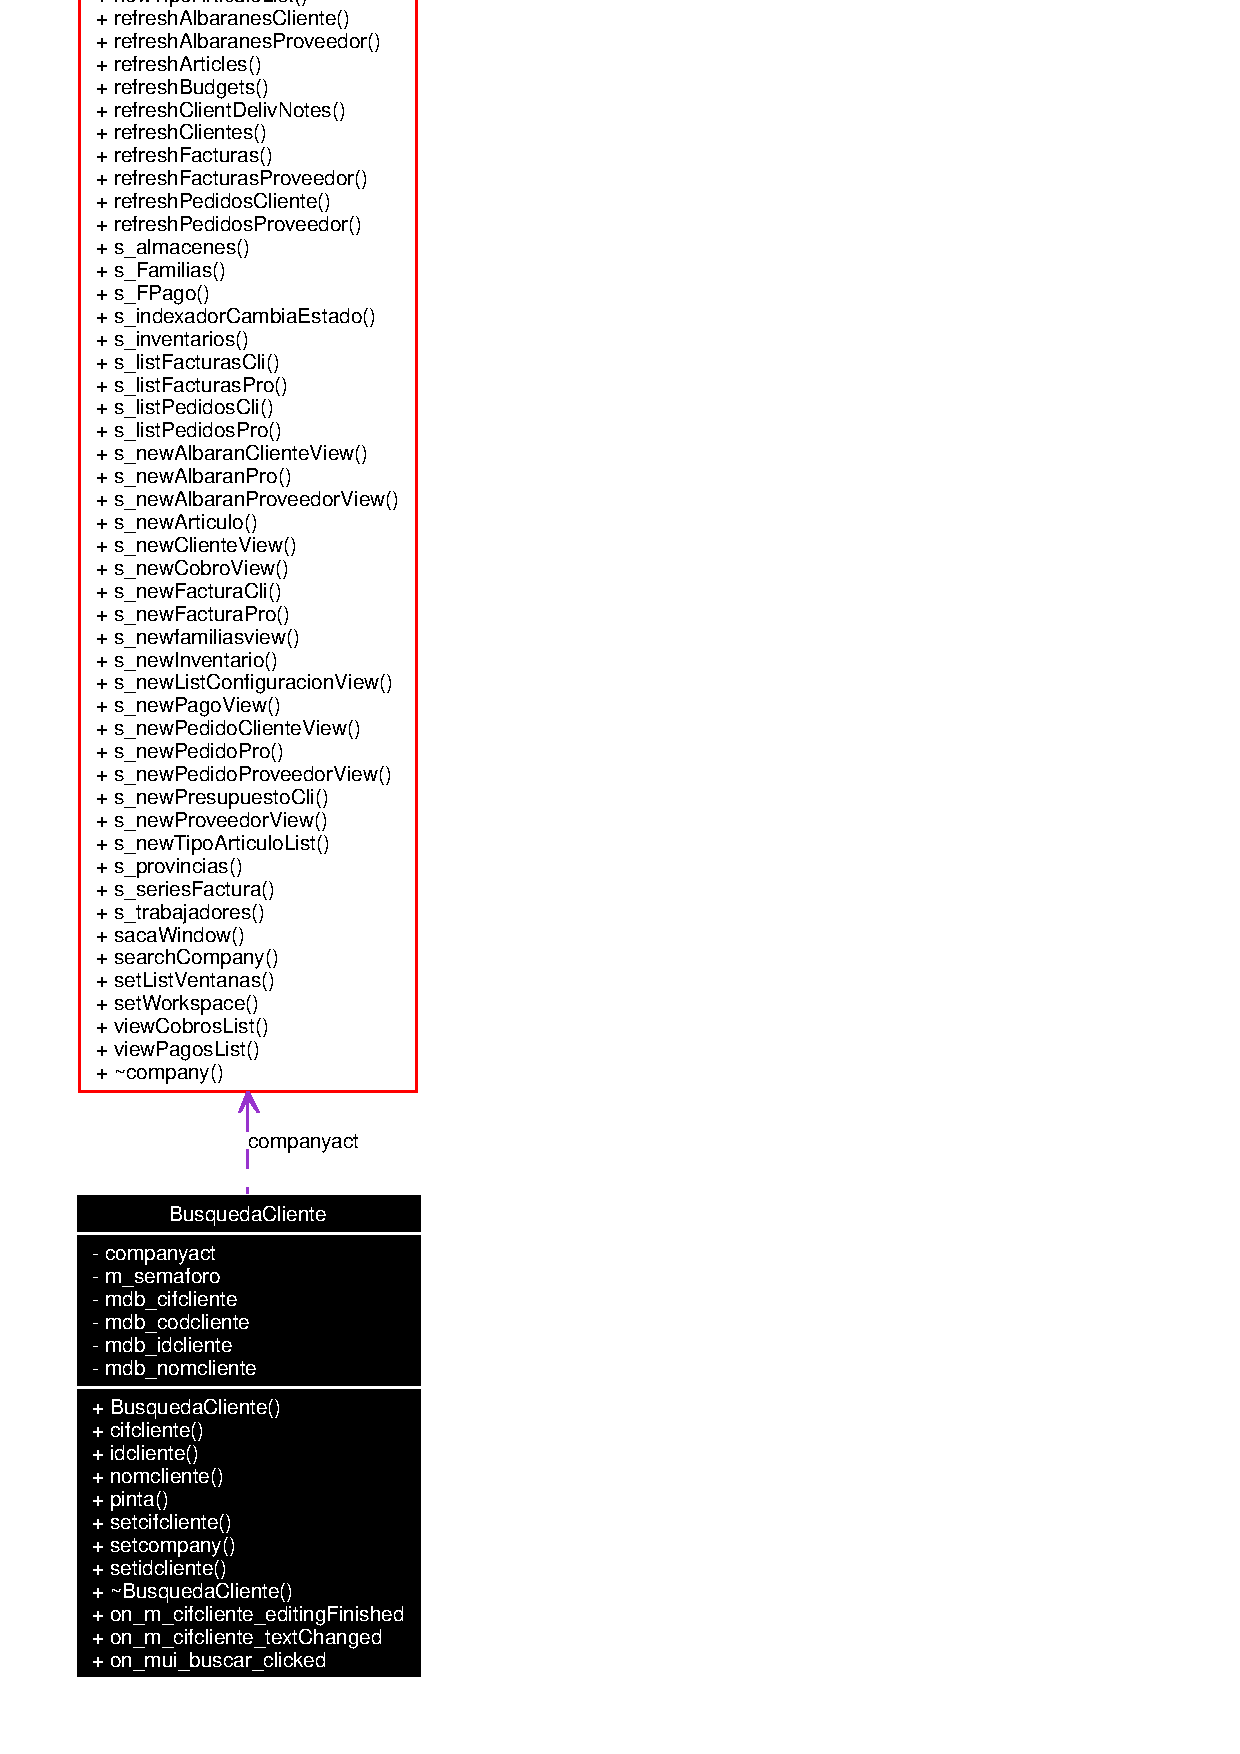
\includegraphics[width=101pt]{classBusquedaCliente__coll__graph}
\end{center}
\end{figure}
\subsection*{Slots p\'{u}blicos}
\begin{CompactItemize}
\item 
virtual void {\bf on\_\-m\_\-cifcliente\_\-editing\-Finished} ()\label{classBusquedaCliente_i0}

\item 
virtual void {\bf on\_\-m\_\-cifcliente\_\-text\-Changed} (const QString \&)\label{classBusquedaCliente_i1}

\item 
virtual void {\bf on\_\-mui\_\-buscar\_\-clicked} ()\label{classBusquedaCliente_i2}

\begin{CompactList}\small\item\em Busqueda de clientes. \item\end{CompactList}\end{CompactItemize}
\subsection*{Se\~{n}ales}
\begin{CompactItemize}
\item 
void {\bf value\-Changed} (QString)\label{classBusquedaCliente_l0}

\end{CompactItemize}
\subsection*{M\'{e}todos p\'{u}blicos}
\begin{CompactItemize}
\item 
{\bf Busqueda\-Cliente} (QWidget $\ast$parent=0)\label{classBusquedaCliente_a0}

\item 
virtual QString {\bf cifcliente} ()\label{classBusquedaCliente_a1}

\item 
virtual QString {\bf idcliente} ()\label{classBusquedaCliente_a2}

\item 
virtual QString {\bf nomcliente} ()\label{classBusquedaCliente_a3}

\item 
void {\bf pinta} ()\label{classBusquedaCliente_a4}

\item 
virtual void {\bf setcifcliente} (QString val)\label{classBusquedaCliente_a5}

\item 
void {\bf setcompany} ({\bf company} $\ast$comp)\label{classBusquedaCliente_a6}

\item 
virtual void {\bf setidcliente} (QString val)\label{classBusquedaCliente_a7}

\end{CompactItemize}


\subsection{Descripci\'{o}n detallada}
Permite buscar y seleccionar un cliente. 

Muestra la parte del formulario que permite buscar y seleccionar un cliente. 



La documentaci\'{o}n para esta clase fu\'{e} generada a partir de los siguientes archivos:\begin{CompactItemize}
\item 
busquedacliente.h\item 
busquedacliente.cpp\end{CompactItemize}
